%%%%%%%%%%%%%%%%%%%%%%%%%%%%%%%%%%%%%%%%%%%%%%%%%%%%%%%%%%%%
%%  This Beamer template was created by Cameron Bracken.
%%  Anyone can freely use or modify it for any purpose
%%  without attribution.
%%
%%  Last Modified: January 9, 2009
%%

\documentclass[xcolor=x11names,compress]{beamer}

%% General document %%%%%%%%%%%%%%%%%%%%%%%%%%%%%%%%%%
\usepackage{graphicx}
\usepackage{tikz}
\usepackage[canadian]{babel}
\usepackage[utf8]{inputenc}
\usepackage{amsmath,amssymb}
\usepackage{mathtools}
\usepackage[ruled,vlined,linesnumbered]{algorithm2e}
\usepackage{epstopdf}
\usepackage{hyperref}
\usepackage[export]{adjustbox}
\usepackage{animate}
\usepackage{minted}
\usepackage{xcolor}
\usepackage{pgfplots}
\usetikzlibrary{calc}
\graphicspath{{img/}}
%%%%%%%%%%%%%%%%%%%%%%%%%%%%%%%%%%%%%%%%%%%%%%%%%%%%%%

\DeclareMathOperator*{\argmax}{arg\,max}
\DeclareMathOperator*{\argmin}{arg\,min}
%% Beamer Layout %%%%%%%%%%%%%%%%%%%%%%%%%%%%%%%%%%
\useoutertheme[subsection=false,shadow]{miniframes}
\useinnertheme{default}
\usefonttheme{serif}
\usepackage{palatino}
\urlstyle{same}
\setbeamerfont{title like}{shape=\scshape}
\setbeamerfont{frametitle}{shape=\scshape}

\setbeamercolor*{lower separation line head}{bg=DeepSkyBlue4} 
\setbeamercolor*{normal text}{fg=black,bg=white} 
\setbeamercolor*{alerted text}{fg=red} 
\setbeamercolor*{example text}{fg=black} 
\setbeamercolor*{structure}{fg=black} 
 
\setbeamercolor*{palette tertiary}{fg=black,bg=black!10} 
\setbeamercolor*{palette quaternary}{fg=black,bg=black!10} 

\renewcommand{\(}{\begin{columns}}
\renewcommand{\)}{\end{columns}}
\newcommand{\<}[1]{\begin{column}{#1}}
\renewcommand{\>}{\end{column}}
\setbeamertemplate{navigation symbols}{}

\setbeamerfont{footline}{size=\fontsize{6}{0}\selectfont}
\setbeamercolor{footline}{fg=black!50}

\setbeamertemplate{footline}{
	\parbox{\paperwidth}{\hspace*{5pt}\url{http://www.cs.toronto.edu/~frossard}\hfill
		\insertframenumber/\inserttotalframenumber\hspace*{5pt}}
	}
\usemintedstyle{tango}
%%%%%%%%%%%%%%%%%%%%%%%%%%%%%%%%%%%%%%%%%%%%%%%%%%

\begin{document}
%%%%%%%%%%%%%%%%%%%%%%%%%%%%%%%%%%%%%%%%%%%%%%%%%%%%%%
%%%%%%%%%%%%%%%%%%%%%%%%%%%%%%%%%%%%%%%%%%%%%%%%%%%%%%
\section{\scshape Introduction}
\begin{frame}
	\title{Introduction to Machine Learning}
	\subtitle{Training Neural Networks}
	\author{
		Davi Frossard\\
		{\it Federal University of Espirito Santo \\ University of Toronto}\\
	}
	\date{
		\vspace{-2em}\\
		\includegraphics[width=0.4\columnwidth]{mlhipster}\\[-1ex]
		{\tiny Credit: {\itshape \url{https://twitter.com/ML_Hipster/status/699758866356015105}}}
		\\
		\today
	}
	\titlepage
\end{frame}

%%%%%%%%%%%%%%%%%%%%%%%%%%%%%%%%%%%%%%%%%%%%%%%%%%%%%%
%%%%%%%%%%%%%%%%%%%%%%%%%%%%%%%%%%%%%%%%%%%%%%%%%%%%%%
\begin{frame}{Summary}
	\tableofcontents
\end{frame}

%%%%%%%%%%%%%%%%%%%%%%%%%%%%%%%%%%%%%%%%%%%%%%%%%%%%%%
%%%%%%%%%%%%%%%%%%%%%%%%%%%%%%%%%%%%%%%%%%%%%%%%%%%%%%
\section{\scshape Backpropagation}
\begin{frame}{Backpropagation}
	\begin{itemize}
		\item So far we've trained models in which we can specify the real error for all the weights.
	\end{itemize}
	\begin{center}
		\begin{tikzpicture}[shorten >=1pt,->,draw=black!50, node distance=\layersep]
			\tikzstyle{every pin edge}=[<-,shorten <=1pt]
			\tikzstyle{neuron}=[circle,draw=black!25,minimum size=17pt,inner sep=0pt]
			\tikzstyle{input neuron}=[neuron, fill=yellow!50];
			\tikzstyle{hidden neuron}=[neuron, fill=green!75];
			\tikzstyle{output neuron}=[neuron, fill=orange!50];
			\tikzstyle{annot} = [text width=4em, text centered]

			\foreach \name / \y in {1,...,4}
			\node[input neuron, pin=left:$x^{(i)}_\y$] (I-\name) at (0,-\y) {};

			\foreach \name / \y in {1,...,5}
			\path[yshift=0.5cm]
			node[output neuron, pin={[pin edge={->}]right:$y^{(i)}_\y$}] (O-\name) at (2*\layersep,-\y cm) {};

			\foreach \source in {1,...,4}
			\foreach \dest in {1,...,5}
			\path (I-\source) edge (O-\dest);
			\node[annot,above of=O-1, node distance=1cm, red!80] (ol) {$logP(y|x,w)$};
		\end{tikzpicture}
	\end{center}
\end{frame}

%%%%%%%%%%%%%%%%%%%%%%%%%%%%%%%%%%%%%%%%%%%%%%%%%%%%%%
%%%%%%%%%%%%%%%%%%%%%%%%%%%%%%%%%%%%%%%%%%%%%%%%%%%%%%
\begin{frame}{Backpropagation}
	\begin{itemize}
		\item What about neural networks?
		      \begin{itemize}
		      	\item<2-> High level view
		      \end{itemize}
	\end{itemize}
	\begin{center}
		\resizebox{0.9\columnwidth}{!}{
			\begin{tikzpicture}[shorten >=1pt,->,draw=black!50, node distance=\layersep]
				\tikzstyle{every pin edge}=[<-,shorten <=1pt]
				\tikzstyle{neuron}=[circle,draw=black!25,minimum size=17pt,inner sep=0pt]
				\tikzstyle{input neuron}=[neuron, fill=green!50];
				\tikzstyle{hidden neuron}=[neuron, fill=blue!50];
				\tikzstyle{output neuron}=[neuron, fill=red!50];
				\tikzstyle{annot} = [text width=4em, text centered]

				\foreach \name / \y in {1,...,4}
				\node[input neuron, pin=left:$x^{(i)}_\y$] (I-\name) at (0,-\y) {};

				\foreach \name / \y in {1,...,5}
				\path[yshift=0.5cm]
				node[hidden neuron] (H1-\name) at (\layersep,-\y cm) {$\sigma$};

				\foreach \source in {1,...,4}
				\foreach \dest in {1,...,5}
				\path (I-\source) edge (H1-\dest);

				\foreach \name / \y in {1,...,6}
				\path[yshift=1.0cm]
				node[hidden neuron] (H2-\name) at (2*\layersep,-\y cm) {$\sigma$};

				\foreach \source in {1,...,5}
				\foreach \dest in {1,...,6}
				\path (H1-\source) edge (H2-\dest);

				\uncover<-3>{\foreach \name / \y in {1,...,5}
					\path[yshift=0.5cm]
					node[output neuron] (O-\name) at (3*\layersep,-\y cm) {};}

				\uncover<1,3->{\foreach \name / \y in {1,...,5}
					\path[yshift=0.5cm]
					node[output neuron, pin={[pin edge={->}]right:$y^{(i)}_\y$}] (O-\name) at (3*\layersep,-\y cm) {};}

				\foreach \source in {1,...,6}
				\foreach \dest in {1,...,5}
				\path (H2-\source) edge (O-\dest);

				\uncover<4>{\draw[red!70,->,line width=3mm] (O-3) -- (O-3-|H2-2.east) node[midway,fill=white] {\emph{BP}};}
				\uncover<5>{\draw[red!70,->,line width=3mm] (O-3) -- (O-3-|H1-2.east) node[midway,fill=white] {\emph{Backward Pass}};}
				\uncover<6>{\draw[red!70,->,line width=3mm] (O-3) -- (O-3-|I-2.east) node[midway,fill=white] {\emph{Backward Pass}};}
				\uncover<2-3>{\draw[blue!70,->,line width=3mm] (O-3-|I-2.east) -- (O-3) node[midway,fill=white] {\emph{Forward Pass}};}
				\uncover<5->{\node[red!80,annot,above of=H2-1, node distance=1cm] (hl2) {$\frac{\partial logP(y|x,w)}{\partial w_{H2}}$};}
				\uncover<6->{\node[red!80,annot,left of=hl2] (hl1) {$\frac{\partial logP(y|x,w)}{\partial w_{H1}}$};}
				\uncover<4->{\node[red!80,annot,right of=hl2] {$\frac{\partial logP(y|x,w)}{\partial w_{out}}$};}
				\uncover<-1>{\node[red!80,annot,above of=H2-1, node distance=1cm] (hl2) {\textbf{?}};}
				\uncover<-1>{\node[red!80,annot,left of=hl2] (hl1) {\textbf{?}};}
				\uncover<-1>{\node[red!80,annot,right of=hl2] {$logP(y|x,w)$};}
			\end{tikzpicture}}
	\end{center}
\end{frame}

%%%%%%%%%%%%%%%%%%%%%%%%%%%%%%%%%%%%%%%%%%%%%%%%%%%%%%
%%%%%%%%%%%%%%%%%%%%%%%%%%%%%%%%%%%%%%%%%%%%%%%%%%%%%%
\begin{frame}{Backpropagation}
	\begin{itemize}
		\item Essentially, we want to extract gradients from the error function to each parameter in the network.
		\item \textit{Neural Network Function}:
		      \begin{gather*}
		      	F(X,W) = \sigma(W_{out}^T\sigma(W_{H2}^T\sigma(W_{H1}^TX)))
		      \end{gather*}
		\item As long as the non-linearities are differentiable, we can estimate the gradients from the function to any of the parameters.
		\item Therefore we can also find the gradients from the error function and minimize it.
	\end{itemize}
\end{frame}

\begin{frame}{Backpropagation}
	\begin{center}
		\begin{tikzpicture}[shorten >=1pt,->,draw=black!50, node distance=\layersep]
			\tikzstyle{every pin edge}=[<-,shorten <=1pt]
			\tikzstyle{neuron}=[circle,draw=black!25,minimum size=17pt,inner sep=0pt]
			\tikzstyle{note}=[draw=black!25,fill=yellow!10,minimum size=15pt,inner sep=0pt]
			\tikzstyle{input neuron}=[neuron, fill=green!50];
			\tikzstyle{hidden neuron}=[neuron, fill=blue!50];
			\tikzstyle{output neuron}=[neuron, fill=red!50];
			\tikzstyle{annot} = [text width=4em, text centered]

			\foreach \name / \y in {1,...,4}
			\node[input neuron, pin=left:$x^{(i)}_\y$] (I-\name) at (0,-\y) {$z^i_\name$};

			\foreach \name / \y in {1,...,5}
			\path[yshift=0.5cm]
			node[hidden neuron] (H1-\name) at (\layersep,-\y cm) {$z^1_\name$};



			\foreach \source in {1,...,4}
			\foreach \dest in {1,...,5}
			\path (I-\source) edge (H1-\dest);

			\foreach \name / \y in {1,...,6}
			\path[yshift=1.0cm]
			node[hidden neuron] (H2-\name) at (2*\layersep,-\y cm) {$z^2_\name$};


			\foreach \source in {1,...,5}
			\foreach \dest in {1,...,6}
			\path (H1-\source) edge (H2-\dest);

			\foreach \name / \y in {1,...,5}
			\path[yshift=0.5cm]
			node[output neuron, pin={[pin edge={->}]right:$y^{(i)}_\y$}] (O-\name) at (3*\layersep,-\y cm) {$z^s_\name$};



			\foreach \source in {1,...,6}
			\foreach \dest in {1,...,5}
			\path (H2-\source) edge (O-\dest);

			\uncover<-1>{\node[note, left of=H1-1, node distance=1cm] (a1) {$a^1_1$};}
			\uncover<-2>{\node[note, left of=H2-1, node distance=1cm] (a2) {$a^2_1$};}
			\uncover<-3>{\node[note, left of=O-1, node distance=1cm] (a3) {$a^s_1$};}

			\uncover<2->{\node[note, left of=H1-1, node distance=1cm] (a12) {$a^1_1+\delta$};}
			\uncover<3->{\node[note, left of=H2-1, node distance=1.2cm] (a22) {$a^2_1+\delta \frac{\partial a^2_1}{\partial a^1_1}$};}
			\uncover<4->{\node[note, left of=O-1, node distance=1.2cm] (a22) {$a^s_1+\delta \frac{\partial a^s_1}{\partial a^1_1}$};}

			\node[annot,above of=H2-1, node distance=1cm] (hl2) {Hidden layer 2};
			\node[annot,left of=hl2] (hl1) {Hidden layer 1};
			\node[annot,left of=hl1] (il1) {Input layer};
			\node[annot,right of=hl2] {Output layer};
		\end{tikzpicture}\vspace{-1ex}
		\begin{itemize}
			\item<5-> Variations are propagated forward!
		\end{itemize}
	\end{center}
\end{frame}

%%%%%%%%%%%%%%%%%%%%%%%%%%%%%%%%%%%%%%%%%%%%%%%%%%%%%%
%%%%%%%%%%%%%%%%%%%%%%%%%%%%%%%%%%%%%%%%%%%%%%%%%%%%%%
\begin{frame}{Backpropagation}
	\begin{itemize}
		\item We need to determine $\delta$ such that the variation propagated forward reduces the error.
		\item In order to do that we work backwards, first calculating the variation we want in the error and {\scriptsize \textit{back}}propagating it to the weights
		\item Using the same notation as before we have:
		      \begin{gather*}
		      	y = \sigma(z^s)\\
		      	E = \hat{y}.log(y)
		      \end{gather*}
	\end{itemize}
\end{frame}

%%%%%%%%%%%%%%%%%%%%%%%%%%%%%%%%%%%%%%%%%%%%%%%%%%%%%%
%%%%%%%%%%%%%%%%%%%%%%%%%%%%%%%%%%%%%%%%%%%%%%%%%%%%%%
\begin{frame}{Backpropagation}
	\begin{alignat*}{2}
		\onslide<1->{\frac{\partial E}{\partial w^s} & = \frac{\partial E}{\partial z^s} \frac{\partial z^s}{\partial w^s}}                                                                                   \\
		\onslide<2->{                                & = (y-z^s)\frac{\partial z^s}{\partial w^s}}
		\only<3>{\intertext{note: $z^s = {w^s}^T\sigma(z^2)$}}
		\onslide<4->{\\&= (y-z^s).\sigma(z^2)}\\
		\onslide<5->{\frac{\partial E}{\partial w^2} & = \frac{\partial E}{\partial z^s} \frac{\partial z^s}{\partial \sigma(z^2)}\frac{\partial \sigma(z^2)}{\partial z^2}\frac{\partial z^2}{\partial w^2}} \\
		\onslide<6->{                                & = (y-z^s)\frac{\partial z^s}{\partial \sigma(z^2)}\frac{\partial \sigma(z^2)}{\partial z^2}\frac{\partial z^2}{\partial w^2}}
		\only<7>{\intertext{$z^s = {w^s}^T\sigma(z^2)$}}
		\onslide<8->{\\&= (y-z^s).w^s\frac{\partial \sigma(z^2)}{\partial z^2}\frac{\partial z^2}{\partial w^2}}\\
		\onslide<9->{                                & = (y-z^s).w^s.\sigma'(z^2)\frac{\partial z^2}{\partial w^2}}
		\only<10>{\intertext{$z^2 = {w^2}^T\sigma(z^1)$}}
		\onslide<11->{\\&= (y-z^s).w^s.\sigma'(z^2).\sigma(z^1)}\\
	\end{alignat*}
\end{frame}

%%%%%%%%%%%%%%%%%%%%%%%%%%%%%%%%%%%%%%%%%%%%%%%%%%%%%%
%%%%%%%%%%%%%%%%%%%%%%%%%%%%%%%%%%%%%%%%%%%%%%%%%%%%%%
\begin{frame}{Backpropagation}
	\begin{alignat*}{2}
		\onslide<1->{\frac{\partial E}{\partial w^1} & = \frac{\partial E}{\partial z^s} \frac{\partial z^s}{\partial \sigma(z^2)}\frac{\partial \sigma(z^2)}{\partial z^2}\frac{\partial z^2}{\partial \sigma(z_1)}\frac{\partial \sigma(z^1)}{\partial z_1}\frac{\partial z^1}{\partial w_1}} \\
		\onslide<2->{                                & = (y-z^s).w^s.\sigma'(z^2)\frac{\partial z^2}{\partial \sigma(z_1)}\frac{\partial \sigma(z^1)}{\partial z_1}\frac{\partial z^1}{\partial w_1}}
		\only<3>{\intertext{$z^2 = {w^2}^T\sigma(z^1)$}}
		\onslide<4->{\\&= (y-z^s).w^s.\sigma'(z^2).w^2\frac{\partial \sigma(z^1)}{\partial z_1}\frac{\partial z^1}{\partial w_1}}\\
		\onslide<5->{                                & = (y-z^s).w^s.\sigma'(z^2).w^2.\sigma'(z_1)\frac{\partial z^1}{\partial w_1}}
		\only<6>{\intertext{$z^1 = {w^1}^Tx$}}
		\onslide<7->{\\&= (y-z^s).w^s.\sigma'(z^2).w^2.\sigma'(z_1).x}
	\end{alignat*}
\end{frame}

%%%%%%%%%%%%%%%%%%%%%%%%%%%%%%%%%%%%%%%%%%%%%%%%%%%%%%
%%%%%%%%%%%%%%%%%%%%%%%%%%%%%%%%%%%%%%%%%%%%%%%%%%%%%%
\begin{frame}{Backpropagation}
	\begin{itemize}
		\item Since we know the gradient of the error function to all the weights, we can use gradient descent to learn the model!
		\item The method is not without faults. Very deep models may experience vanishing or exploding gradients
		      \begin{itemize}
		      	\item More on that when we see Recurrent Neural Networks.
		      \end{itemize}
	\end{itemize}
\end{frame}

%%%%%%%%%%%%%%%%%%%%%%%%%%%%%%%%%%%%%%%%%%%%%%%%%%%%%%
%%%%%%%%%%%%%%%%%%%%%%%%%%%%%%%%%%%%%%%%%%%%%%%%%%%%%%
\section{\scshape Challenges}
\subsection{Underfit}
\begin{frame}{Training Challenges}
	\begin{itemize}
		\item During training, you might find that your model is underfitting, which most of the times means that your model is too simple for the data you're trying to fit.
		      \begin{itemize}
		      	\item Either change the training method;
		      	\item Or use a more complex model (more hidden layers, for instance).
		      \end{itemize}
		      \only<2>{\begin{center}
		      	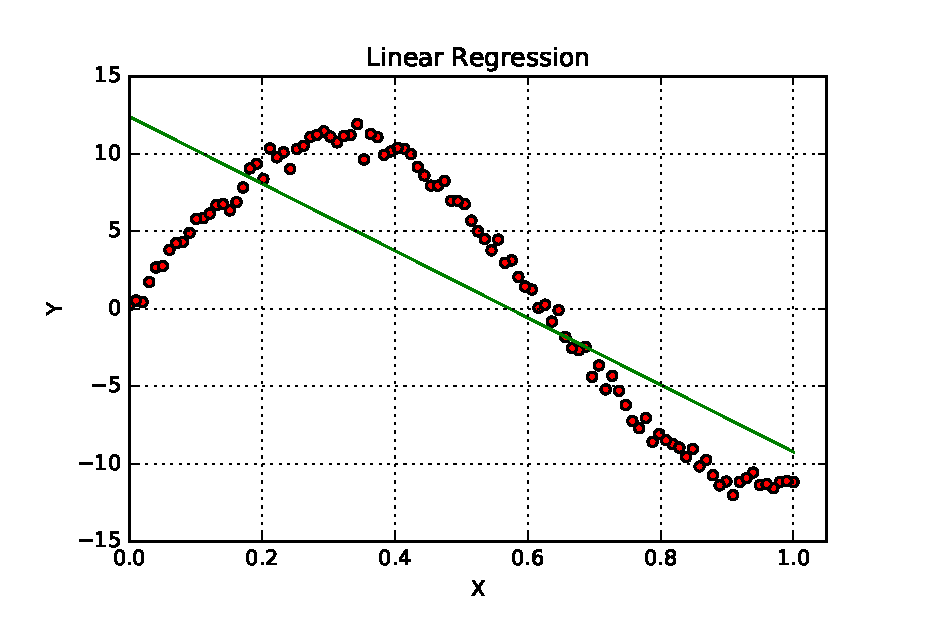
\includegraphics[width=0.7\columnwidth]{underfit}
		      	\end{center}}
	\end{itemize}
\end{frame}

%%%%%%%%%%%%%%%%%%%%%%%%%%%%%%%%%%%%%%%%%%%%%%%%%%%%%%
%%%%%%%%%%%%%%%%%%%%%%%%%%%%%%%%%%%%%%%%%%%%%%%%%%%%%%
\subsection{Overfit}
\begin{frame}{Training Challenges}
	\begin{itemize}
		\item While underfit is an issue, most of the times it can be easily solved. The real challenge is in dealing with \textbf{overfit}.
		\item Overfit usually stems from one of these scenarios:
		      \begin{itemize}
		      	\item Big model + Not enough data.
    	      \item<3-> \textit{Unlearnable} data.
						\only<5>{\begin{itemize}
							\item A neural network that writes valid python code?
						\end{itemize}}
		      \end{itemize}
	\end{itemize}
	\only<2>{\begin{center}
		\includegraphics[width=0.6\columnwidth]{overfit}\\[-1ex]
		{\tiny Credit: {\itshape \href{http://www.springer.com/gb/book/9780387310732}{Pattern Recognition and Machine Learning - Cristopher Bishop}}}
		\end{center}}
	\only<4>{\begin{center}
			\includegraphics[width=0.75\columnwidth]{random}\\[-1ex]
			\end{center}}
\end{frame}

%%%%%%%%%%%%%%%%%%%%%%%%%%%%%%%%%%%%%%%%%%%%%%%%%%%%%%
%%%%%%%%%%%%%%%%%%%%%%%%%%%%%%%%%%%%%%%%%%%%%%%%%%%%%%
\begin{frame}{Training Challenges}
	\begin{itemize}
		\item Neural network writing \LaTeX:
	\end{itemize}
	\begin{center}
		\includegraphics[width=\columnwidth]{latex3}\\[-1ex]
		{\tiny Credit: {\itshape \url{http://karpathy.github.io/2015/05/21/rnn-effectiveness/}}}
		\end{center}
\end{frame}

%%%%%%%%%%%%%%%%%%%%%%%%%%%%%%%%%%%%%%%%%%%%%%%%%%%%%%
%%%%%%%%%%%%%%%%%%%%%%%%%%%%%%%%%%%%%%%%%%%%%%%%%%%%%%
\subsection{Regularization}
\begin{frame}{Regularization}
	\begin{itemize}
		\item One way to deal with overfit is with \textbf{regularization}.
		\item Consists in introducing additional information to the model based on prior belief about how the parameters should behave.
		\item In general its a term added to the objective function.
		\begin{gather*}
			O(x,y,w) = \sum \alpha E(x,y) + \lambda R(w)
		\end{gather*}
	\end{itemize}
\end{frame}

%%%%%%%%%%%%%%%%%%%%%%%%%%%%%%%%%%%%%%%%%%%%%%%%%%%%%%
%%%%%%%%%%%%%%%%%%%%%%%%%%%%%%%%%%%%%%%%%%%%%%%%%%%%%%
\subsubsection{L2 Regularization}
\begin{frame}{L2 Regularization}
	\begin{itemize}
		\item One such term is L2 Regularization:
		\begin{gather*}
			R(w) = w^2
		\end{gather*}
		\item Favors small but non-zero weights.
		\item Produces smoother models.
		\item \textit{Usually} the best for classification.
		\item Same as a Gaussian Prior on the weights.
	\end{itemize}
	\begin{center}
		\includegraphics[width=0.7\columnwidth]{reg_strengths}\\[-1ex]
		{\tiny Credit: {\itshape \url{http://cs231n.github.io/neural-networks-1/}}}
		\end{center}
\end{frame}

%%%%%%%%%%%%%%%%%%%%%%%%%%%%%%%%%%%%%%%%%%%%%%%%%%%%%%
%%%%%%%%%%%%%%%%%%%%%%%%%%%%%%%%%%%%%%%%%%%%%%%%%%%%%%
\subsubsection{L1 Regularization}
\begin{frame}{L1 Regularization}
	\begin{itemize}
		\item There is also L1 Regularization:
		\begin{gather*}
			R(w) = |w|
		\end{gather*}
		\item Favors sparsity (easier to set weights to 0).
		\item Allows feature selection.
		\item Same as a Laplace Prior on the weights.
	\end{itemize}
	\begin{center}
		\includegraphics[width=0.7\columnwidth]{Sparsityl1}\\[-1ex]
		{\tiny Credit: {\itshape \url{https://en.wikipedia.org/wiki/Regularization_(mathematics)}}}
	\end{center}
\end{frame}

%%%%%%%%%%%%%%%%%%%%%%%%%%%%%%%%%%%%%%%%%%%%%%%%%%%%%%
%%%%%%%%%%%%%%%%%%%%%%%%%%%%%%%%%%%%%%%%%%%%%%%%%%%%%%
\subsubsection{Example}
\begin{frame}{Tangible Example}
	\begin{itemize}
		\item Suppose we want to predict shoe size given height and weight. Also, lets assume that its easier to predict shoe size from height than from weight.
		\item L1 Regularization:
		\uncover<2->{
		\begin{itemize}
			\item Set the weight feature \textbf{W} to zero and learn the ratio between shoe size and height.
		\end{itemize}
		}
		\item L2 Regularization:
		\uncover<2->{
		\begin{itemize}
			\item Learn positive weights for both weight and height.
		\end{itemize}
		}
	\end{itemize}
\end{frame}

%%%%%%%%%%%%%%%%%%%%%%%%%%%%%%%%%%%%%%%%%%%%%%%%%%%%%%
%%%%%%%%%%%%%%%%%%%%%%%%%%%%%%%%%%%%%%%%%%%%%%%%%%%%%%
\begin{frame}{Tangible Example}
	\begin{itemize}
		\item But why does regularizing help prevent overfit?
		\uncover<2->{
		\begin{itemize}
			\item Makes it difficult for uncommon features to have very large weights (L2) or simply exclude the feature from the model (L1).
		\end{itemize}
		}
	\end{itemize}
\end{frame}

%%%%%%%%%%%%%%%%%%%%%%%%%%%%%%%%%%%%%%%%%%%%%%%%%%%%%%
%%%%%%%%%%%%%%%%%%%%%%%%%%%%%%%%%%%%%%%%%%%%%%%%%%%%%%
\subsection{Dropout}
\begin{frame}{Dropout}
\begin{itemize}
	\item Another method used to prevent overfitting is \textbf{Dropout}.
	\item Intuitively, it works by breaking down a big network into smaller sub-networks and learning them 'independently', with the final model being the combination of the learned smaller models.
	\item It prevents complex co-adaptations of the neurons since sometimes they aren't allowed to cooperate.
\end{itemize}
\end{frame}

%%%%%%%%%%%%%%%%%%%%%%%%%%%%%%%%%%%%%%%%%%%%%%%%%%%%%%
%%%%%%%%%%%%%%%%%%%%%%%%%%%%%%%%%%%%%%%%%%%%%%%%%%%%%%
\begin{frame}{Dropout}
	\begin{tikzpicture}[shorten >=1pt,->,draw=black!50, node distance=\layersep, cross/.style={path picture={
			\draw[black, thick]
			(path picture bounding box.south east) -- (path picture bounding box.north west) (path picture bounding box.south west) -- (path picture bounding box.north east);
		}}]
		\tikzstyle{every pin edge}=[<-,shorten <=1pt]
		\tikzstyle{neuron}=[circle,draw=black!25,minimum size=17pt,inner sep=0pt]
		\tikzstyle{input neuron}=[neuron, fill=green!50];
		\tikzstyle{hidden neuron}=[neuron, fill=blue!50];
		\tikzstyle{output neuron}=[neuron, fill=red!50];
		\tikzstyle{dropout neuron}=[neuron, fill=gray!50];
		\tikzstyle{annot} = [text width=4em, text centered]

		\foreach \name / \y in {1,...,4}
		\node[input neuron, pin=left:$x^{(i)}_\y$] (I-\name) at (0,-\y) {};

		\foreach \name / \y in {1,3,5}
		\path[yshift=0.5cm]
		node[hidden neuron] (H1-\name) at (\layersep,-\y cm) {$\sigma$};

		\foreach \name / \y in {2,4}
		\path[yshift=0.5cm]
		node[dropout neuron, cross] (H1-\name) at (\layersep,-\y cm) {};

		\foreach \source in {1,...,4}
		\foreach \dest in {1,3,5}
		\path (I-\source) edge (H1-\dest);

		\foreach \name / \y in {1,3,4,6}
		\path[yshift=1.0cm]
		node[hidden neuron] (H2-\name) at (2*\layersep,-\y cm) {$\sigma$};

		\foreach \name / \y in {2,5}
		\path[yshift=1.0cm]
		node[dropout neuron, cross] (H2-\name) at (2*\layersep,-\y cm) {};

		\foreach \source in {1,3,5}
		\foreach \dest in {1,3,4,6}
		\path (H1-\source) edge (H2-\dest);

		\foreach \name / \y in {1,...,5}
		\path[yshift=0.5cm]
		node[output neuron, pin={[pin edge={->}]right:$y^{(i)}_\y$}] (O-\name) at (3*\layersep,-\y cm) {};

		\foreach \source in {1,3,4,6}
		\foreach \dest in {1,...,5}
		\path (H2-\source) edge (O-\dest);
	\end{tikzpicture}
\end{frame}

%%%%%%%%%%%%%%%%%%%%%%%%%%%%%%%%%%%%%%%%%%%%%%%%%%%%%%
%%%%%%%%%%%%%%%%%%%%%%%%%%%%%%%%%%%%%%%%%%%%%%%%%%%%%%
\begin{frame}{Dropout}
\begin{itemize}
	\item During training time:
	\begin{itemize}
		\item Unit present with probability $p$.
	\end{itemize}
	\item During test time:
	\begin{itemize}
		\item Unit always present, weight multiplied by $p$.
	\end{itemize}
\end{itemize}
\end{frame}


\end{document}
